% begin module exponential-versus-polynomial
\begin{frame}
\begin{center}
\small
Graphical comparison of $y = 2^x$ with $y = x^2$. Axes have different scales.
\begin{tabular}{cc}
\uncover<1->{
\psset{xunit=0.8cm, yunit=0.1cm}
\begin{pspicture}(-5, -5)(5,5) 
\psframe*[linecolor=white](-5,-5)(5,5) 
\psaxes[ticks=x, labels=x]{<->}(0,0)(-1,-3)(5.01,60)
\psline(-0.1,40)(0.1, 40)
\rput[l](0.2, 40){$40$} 
\psline(-0.1,20)(0.1, 20)
\rput[l](0.2, 20){$20$} 
%Function formula: 2^{x} 
\psplot[linecolor=red, plotpoints=1000]{-0.5}{5}{2 x exp }
\psplot[linecolor=blue, plotpoints=1000]{-0.5}{5}{x 2 exp }
\end{pspicture}
%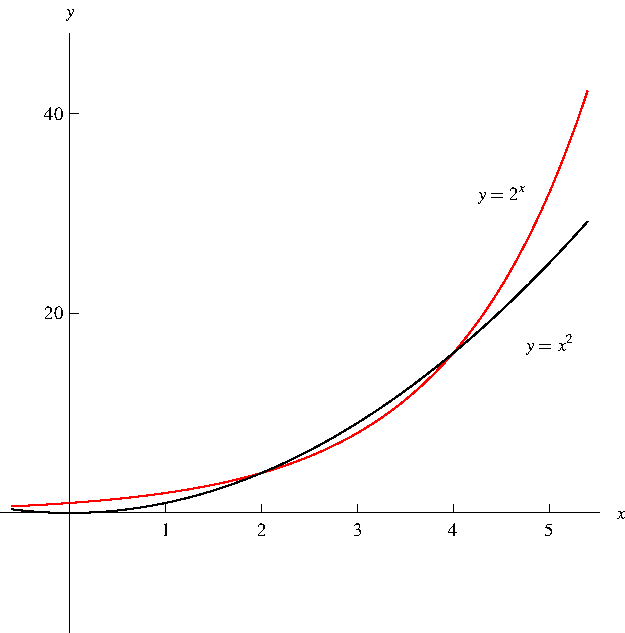
\includegraphics[height=5cm]{exponential-functions/pictures/07-02-expvspowera.pdf}%
}
&%
\uncover<2->{
\psset{xunit=0.25cm, yunit=0.05cm}
\begin{pspicture}(-5, -5)(5,5) 
\psframe*[linecolor=white](-5,-5)(5,5) 
\psaxes[ticks=x, Dx=4, labels=x]{<->}(0,0)(-1,-8)(16,120)
\psline(-0.4,100)(0.4, 100)
\rput[l](0.6, 100){$100$} 
%Function formula: 2^{x} 
\psplot[linecolor=red, plotpoints=1000]{-0.5}{7}{2 x exp }
\psplot[linecolor=blue, plotpoints=1000]{-0.5}{11.313708499}{x 2 exp }
\psline(-0.5, -3.5)(5, -3.5)(5, 32)(-0.5, 32)(-0.5, -3.5)
\rput[l](6, 10){Magnified region}
\end{pspicture}
%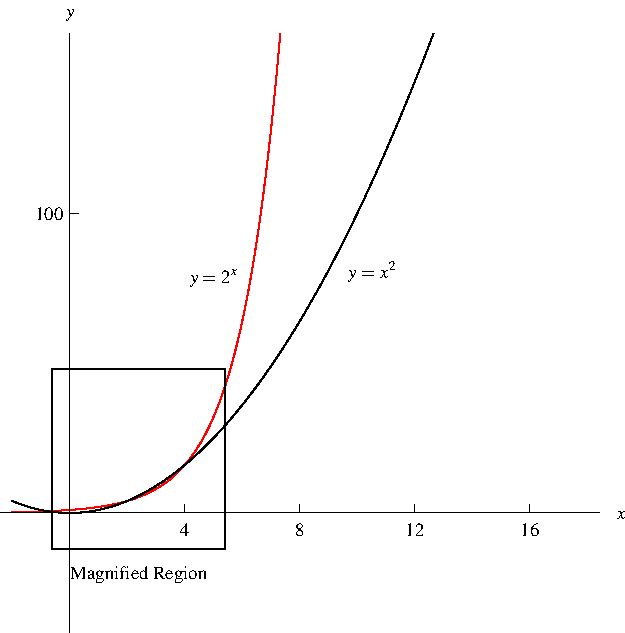
\includegraphics[height=5cm]{exponential-functions/pictures/07-02-expvspowerb.pdf}%
}
\end{tabular}
\end{center}
\end{frame}
% end module exponential-versus-polynomial